\chapter{Estrategia constructiva.}\label{cap:capitulo4}

Hasta ahora hemos visto la representación de las distintas entidades que entran en juego. En este capítulo introduciremos parte de la lógica que seguirá el sistema. Destacar que, aunque el enfoque final ha sido reducir el problema a una modificación de búsqueda, el sistema está pensado de forma que sea flexible a la hora de utilizar otro tipo de estrategias.


\section{Algoritmo de generación}
A la metodología que hemos utilizado la hemos denominado \emph{estrategia constructiva}, cuyo origen radica en la forma de generar el mapa. Como se puede ver en el listado \ref{lst:mlisting}, el sistema construirá el mapa por pasos. de forma que en cada paso se hará una elección de una habitación y se colocará en el mapa. Así, el sistema dará por concluida la generación cuando no queden habitaciones en la lista inicial.

\begin{lstlisting}[caption={Algoritmo constructivo para generar mapas},label={lst:mlisting},language=Java,escapechar=|]
Mapa GenerarMapa( List<Habitacion> habitaciones, InterfazSeleccion mapSolver ) {
	Mapa mapa = MapaVacio();
	while( !habitaciones.isEmpty() ) {
		List<Movimiento> movimientos = GenerarMovimientos( mapa, habitaciones ); |\label{line:movgen}|
		Movimiento elegido = mapSolver.ElegirMovimiento( mapa, movimientos ); |\label{line:ifaceselect}|
		mapa.InsertarHabitacion( elegido.habitacion, elegido.posicion ); |\label{line:addroom}|
		habitaciones.remove( elegido.habitacion ); |\label{line:rmroom}|
		GuardarMovimiento( elegido ); |\label{line:savemov}|
	}
	EstablecerRecorridoPrincipal( mapa ); |\label{line:inifin}|
	return mapa;
}
\end{lstlisting}

En el listado \ref{lst:mlisting} se introducen dos conceptos nuevos: \emph{movimientos} e \emph{interfaz de selección de movimiento}, y ambos son clave para el entendimiento del funcionamiento del sistema.

A grandes rasgos, se elige un par $(habitacion, posicion)$ y se inserta en el mapa (línea~\ref{line:addroom}). Posteriormente, se elimina la habitación de la lista de habitaciones, ya que se acaba de colocar (línea~\ref{line:rmroom}). Por último, guardamos el movimiento (línea~\ref{line:savemov}). Más adelante veremos la utilidad de ésto.

Antes de devolver el mapa, establecemos el recorrido principal (línea~\ref{line:inifin}), es decir, elegimos la habitacion inicial y final. Para ello, se ha empleado el algoritmo de \emph{Floyd-Warshall}, ayudándonos de la \emph{matriz superior de conexiones entre habitaciones} comentada en el capítulo~\ref{cap:capitulo3}. El objetivo del algoritmo \emph{Floyd-Warshall} \cite{floydwarshall} es, dado un grafo, establecer los caminos mínimos entre todos los pares de nodos posibles. Así, para establecer el recorrido principal, elegiremos el par de nodos cuya distancia mínima sea mayor.

\section{Movimientos}

Un movimiento $M_i(R_i,P_i)$ está constituido por:

\begin{itemize}
	\item$R_i$: \emph{instancia de habitación} a colocar en el mapa
	\item$P_i$: \emph{posición} del mapa donde colocaremos dicha habitación
\end{itemize}

Así, en cada paso de colocación de una habitación, se generarán todos los movimientos posibles a realizar (listado~\ref{lst:mlisting}, línea~\ref{line:movgen}). La lista de movimientos posibles dependerá del estado del sistema, como veremos a continuación.

\subsection{Cómputo de posibles movimientos.}

Consideraremos que el \emph{estado del sistema} depende de, y se ve afectado por:

\begin{itemize}
	\item Instancias de habitación restantes en la lista inicial
	\item Modelo de instancias de habitaciones colocadas en el mapa
	\item Posición de las instancias de habitaciones colocadas
\end{itemize}

Como se observa en la figura~\ref{fig:posmovs}, dado un estado del sistema $S(map,RR)$, la lista de posibles movimientos se computará a partir de las \emph{posibles conexiones} entre las \emph{puertas potenciales de las habitaciones colocadas en el mapa} y las \emph{puertas potenciales de las habitaciones restantes}. El concepto de \emph{puerta potencial} se discutió en el capítulo\ref{cap:capitulo3}.

El cómputo de las posibles conexiones entre el mapa y una de las habitaciones restantes, se define en la figura~\ref{fig:poscons}. En la figura~\ref{fig:grafhabmap} se puede ver una ilustración de los tiles implicados. Destacar que el desplazamiento para testear la posible conexión entre una habitación de las restantes y una del mapa, solamente se puede realizar sobre la habitación restante, ya que las del mapa ya han sido colocadas y están fijas.


El cómputo de todos los posibles movimientos queda como la unión de los conjuntos que dan como resultado calcular las posibles conexiones entre todas las habitaciones restantes y las presentes en el mapa.

Así, el cómputo de todas las posibles conexiones entre una habitación en la lista de habitaciones restantes y una habitación del mapa consiste en calcular el conjunto de todas las posibles colocaciones de la habitación de la lista de restantes contigua a la habitación del mapa.


\begin{figure}[h]
\centering
{
	$$S(map, RR), RR = habitacionesRestantes$$
	$$movimientos = \bigcup_{r \in RR}posiblesConexiones(map, r)$$
}
\caption{Cómputo de lista de movimientos dado un estado del sistema
\label{fig:posmovs}
}
\end{figure}



\begin{figure}[H]
	$$posiblesConexiones(map, r) = $$
	$$\bigcup_{p \in rooms(map)}  \left\{ cx(map,r,p,u,v,w) : \neg col(map, r, w) \right\}$$
	$$w = v - u + \begin{cases}
		(-1,0) \\
		(+1,0) \\
		(0,-1) \\
		(0,+1) \\
	\end{cases}$$
	$$u \in r, v \in map, w \in map$$
	$$puertaPotencial(u, r), puertaPotencial(v, p)$$
	$$col(map, room, t) : \text{colisión al colocar $room$ en $map$ en el tile $t$}$$
	$$cx(map,r,p,u,v,w) : \text{conectar $u \in r$ y $u \in p$ colocando $r$ en tile $w \in map$}$$
\caption{Cómputo de las posibles conexiones entre una habitación de las restantes y el mapa
\label{fig:poscons}
}
\end{figure}


\begin{figure}[H]
\centering
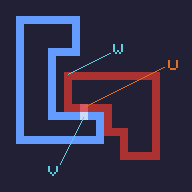
\includegraphics[scale=1]{img/tileconn}
\caption{Ilustración de posible conexión entre habitación y mapa
\label{fig:grafhabmap}}
\end{figure}



\section{Interfaz de selección de movimiento}

Como se ha comentado anteriormente, la \emph{interfaz de selección de movimiento} es otro elemento importante del sistema, y en ella radica parte de la flexibilidad del sistema. En el listado \ref{lst:igen} se muestra el esqueleto de dicha interfaz, cuyo único método de interés es el relacionado con la elección del movimiento.

\begin{lstlisting}[caption={Interfaz de selección de movimiento},label={lst:igen},language=Java,escapechar=|]
interface InterfazSeleccion {
	Movimiento ElegirMovimiento( Mapa mapa, List<Movimiento> movimientos );
}
\end{lstlisting}

Una vez generados todos los movimientos posibles, se delega la decisión de elegir un movimiento a la \emph{interfaz de selección de movimiento}. En esta interfaz radica uno de los puntos de flexibilidad del sistema. Mediante componentes que implementen esta interfaz, podemos idear otras formas de elegir un movimiento a partir de la lista de movimientos posibles.

En este proyecto se han creado dos interfaces de selección de movimiento:

\begin{itemize}
	\item \emph{Interfaz aleatoria}. Elige un movimiento de forma aleatoria de entre todos los posibles.
	\item \emph{Interfaz basada en búsqueda}. Asigna una puntuación a cada movimiento y elige la mejor.
\end{itemize}

La interfaz aleatoria es simple y no tiene interés computacional. En el listado \ref{lst:irandom} se muestra la implementación de dicha interfaz por completitud, pero se ha realizado solo para testeo.

\begin{lstlisting}[caption={Implementación aleatoria de la interfaz de selección de movimiento},label={lst:irandom},language=Java,escapechar=|]
class RandomMovementSelector implements IMovementSelector {
	Movimiento ElegirMovimiento( Mapa mapa, List<Movimiento> movimientos ) {
		int indiceMovimiento = random( 0, movimientos.size() - 1);
		Movimiento elegido = movimientos.get( indiceMovimiento );
		return elegido;
	}
}
\end{lstlisting}

